\chapter{Uitvoeren van pipelines en verzamelen van resultaten}%
\label{ch:uitvoeren}

Voor het vergelijken van de kostprijs en performantie van beide pipelines in Azure Data Factory en Azure Databricks zullen de pipelines op verschillende manieren dagelijks uitgevoerd worden.

\begin{figure}[H]%
    \centering
    \begin{tabularx}{0.9\textwidth}{ |X|X| }
        \hline
        \textbf{Compute Size} & \textbf{Core count} \\
        \hline 
        Small  & 4 Worker Cores + 4 Driver Cores  \\
        \hline
        Medium & 8 Worker Cores + 8 Driver Cores \\
        \hline
    \end{tabularx}
    \caption{Data flow runtimes voor het uitvoeren van de Azure Data Factory pipeline.}
\end{figure}
    
\begin{figure}[H]%  
    \centering
    \begin{tabularx}{0.9\textwidth}{ |X|X|X| }
        \hline
        \textbf{Worker type + Driver type} & \textbf{Core count} & \textbf{Memory} \\
        \hline 
        Standard\_D4ads\_v5 & 4 Worker Cores + 4 Driver Cores & 16GB Worker Memory + 16GB Driver Memory  \\
        \hline
        Standard\_D8ads\_v5 & 8 Worker Cores + 8 Driver Cores & 16GB Worker Memory + 16GB Driver Memory  \\
        \hline
    \end{tabularx}
    \caption{Clusters voor het uitvoeren van de Azure Databricks pipeline.}
\end{figure}

Zowel de Azure Data Factory pipeline als de Azure Databricks pipeline zullen dagelijks gerund worden op twee verschillende compute sizes. Hierbij wordt er telkens gekeken naar ``4 Worker Cores + 4 Driver Cores'' en ``8 Worker Cores + 8 Driver Cores''.

\section{Azure Data Factory}

Het vinden van de kosten voor Azure Data Factory kan in Microsoft Cost Management terug gevonden worden. Hierbij kan er gefilterd worden per dag om de dagelijkse kosten voor het uitvoeren van de pipelines terug te vinden. In Azure Data Factory zelf kan er gekozen worden om een billing report op pipeline of factory level te tonen. Maar doordat er gebruik gemaakt wordt van Azure Data Flow in Azure Data Factory komen de kosten van beide pipelines nog steeds terecht in één enkele resource in het billing report. Hierdoor kan enkel de totale kostprijs voor het uitvoeren van de twee pipelines voor een bepaalde dag gevonden worden. Gelukkig kan in Azure Data Factory zelf de consumption per pipeline gevonden worden. Aan de hand hier van kunnen de kosten voor het uitvoeren van deze pipeline berekend worden.

Een voorbeeld hiervan is dat de totale kostprijs voor Azure Data Factory in het billing report op 5 mei €0,72 bedraagd. Wanneer we in Azure Data Factory naar de consumption per pipeline gaan kijken vinden we het volgende terug:


\begin{figure}[H]
    \centering
    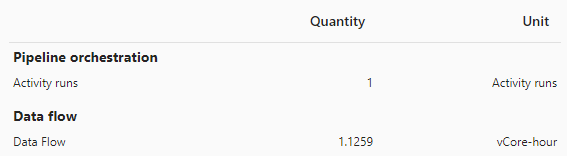
\includegraphics[width=1\textwidth]{./graphics/kosten/5_mei_consumption_small.png}
    \caption{Consumption voor het uitvoeren van de pipeline met 4 Worker Cores + 4 Driver Cores}
\end{figure}

    
\begin{figure}[H]
    \centering
    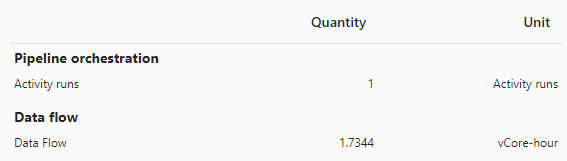
\includegraphics[width=1\textwidth]{./graphics/kosten/5_mei_consumption_medium.png}
    \caption{Consumption voor het uitvoeren van de pipeline met 8 Worker Cores + 8 Driver Cores}
\end{figure}

Beide pipelines hebben één activity run. Doordat de prijs per 1.000 activity runs slechts €0,937 bedraagd betekent dit dat de prijs voor één enkele activity run onder de €0,01 zit. Hierdoor zullen we hier geen rekening mee houden.

Wat wel belangrijk is, is het aantal vCore-hour er verbruikt is in Azure Data Flow. De kostprijs per vCore-hour in Azure Data Flow bedraagd 	€0.251. Aan de hand hier van kunnen we dus de kostprijs per pipeline berekenen:\\


1,1259 vCore-hour x €0.251 = €0,2826009 $\approx$ €0,28\\


1,7344 vCore-hour x €0.251 = €0,4353344 $\approx$ €0,44\\


De kosten voor het uitvoeren van de pipeline met 4 Worker Cores + 4 Driver Cores bedraagd dus €0,28 en voor de pipeline met 8 Worker Cores + 8 Driver Cores bedraagd dit €0,44. Wanneer we deze kosten optellen komen we uit op de eerdere gevonden totale kost van €0,72. Elke dag zal dus de kostprijs op deze manier berekent worden. Ook de tijd die nodig is voor het uitvoeren van een pipeline en de cluster startup tijd vinden we terug in Azure Data Factory. 


\textbf{4 Worker Cores + 4 Driver Cores}

\begin{figure}[H]%  
    \centering
    \begin{tabularx}{1\textwidth}{ |X|X|X|X|X| }
        \hline
        \textbf{Datum} & \textbf{Kost} & \textbf{Totale tijd} & \textbf{Cluster startup tijd} & \textbf{Uitvoeringstijd} \\
        \hline 
        05/05 & € 0,28 & 10m & 3m 11s & 6m 49s  \\
        \hline
        06/05 & € 0,29 & 10m 48s & 2m 57s & 7m 51s \\
        \hline
        07/05 & € 0,29 & 10m 2s & 3m 9s & 6m 53s \\
        \hline
    \end{tabularx}
    \caption{Kost en tijd voor het uitvoeren van de pipeline met 4 Worker Cores + 4 Driver Cores.}
\end{figure}


\textbf{8 Worker Cores + 8 Driver Cores}

\begin{figure}[H]%  
    \centering
    \begin{tabularx}{1\textwidth}{ |X|X|X|X|X| }
        \hline
        \textbf{Datum} & \textbf{Kost} & \textbf{Totale tijd} & \textbf{Cluster startup tijd} & \textbf{Uitvoeringstijd} \\
        \hline 
        05/05 & € 0,44 & 7m 53s & 3m 6s & 4m 47s  \\
        \hline
        06/05 & € 0,47 & 8m 6s & 3m 24s & 4m 42s \\
        \hline
        07/05 & € 0,43 & 7m 56s & 2m 42s & 5m 14s \\
        \hline
    \end{tabularx}
    \caption{Kost en tijd voor het uitvoeren van de pipeline met 8 Worker Cores + 8 Driver Cores.}
\end{figure}

\section{Azure Databricks}

Voor het vinden van de kostprijs voor de pipelines in Azure Databricks zijn er twee Databricks instances aangemaakt. Één voor de pipeline met 4 Worker Cores + 4 Driver Cores en één voor de pipeline met 8 Worker Cores + 8 Driver Cores. Hierdoor kan er in het billing report gekeken worden naar de kosten voor de pipelines appart. Belangrijk om hierbij te vermelden is dat, zoals te zien in figuur~\ref{fig:conf-databricks}, bij het aanmaken van Azure Databricks, er een Managed Resource Group name gekozen kan worden. Aan de hand van deze naam kan er gekeken worden naar de kosten van bijvoorbeeld virtual machines, storage accounts en virtual networks van de pipeline. Al deze kosten optellen voor een bepaalde dag zal dus de totale kost voor het uitvoeren van een pipeline uitkomen. De tijd zelf voor het uitvoeren van de pipelines vinden we terug in Databricks. Hierbij staat er geen cluster startup tijd maar deze kan teruggevonden worden met behulp van de Databricks REST API of Databricks CLI.


\textbf{4 Worker Cores + 4 Driver Cores}

\begin{figure}[H]%  
    \centering
    \begin{tabularx}{1\textwidth}{ |X|X|X|X|X| }
        \hline
        \textbf{Datum} & \textbf{Kost} & \textbf{Totale Tijd} & \textbf{Cluster startup tijd} & \textbf{Uitvoeringstijd} \\
        \hline 
        05/05 & € 0,22 & 10m 44s &  3m 48s & 6m 56s \\
        \hline
        06/05 & € 0,21 & 10m 16s & 3m 45s & 6m 31s \\
        \hline
        07/05 & € 0,21 & 10m 20s & 4m 8s & 6m 12s \\
        \hline
    \end{tabularx}
    \caption{Kost en tijd voor het uitvoeren van de pipeline met 4 Worker Cores + 4 Driver Cores.}
\end{figure}

\textbf{8 Worker Cores + 8 Driver Cores}

\begin{figure}[H]%  
    \centering
    \begin{tabularx}{1\textwidth}{ |X|X|X|X|X| }
        \hline
        \textbf{Datum} & \textbf{Kost} & \textbf{Totale Tijd} & \textbf{Cluster startup tijd} & \textbf{Uitvoeringstijd} \\
        \hline 
        05/05 & € 0,42 & 7m 17s & 3m 22s & 3m 55s \\
        \hline
        06/05 & € 0,42 & 7m 43s & 3m 44s & 3m 59s \\
        \hline
        07/05 & € 0,46 & \textcolor{red}{10m 30s} & \textcolor{red}{6m 27s} & 4m 3s \\
        \hline
    \end{tabularx}
    \caption{Kost en tijd voor het uitvoeren van de pipeline met 8 Worker Cores + 8 Driver Cores.}
\end{figure}

Zoals te zien in de rode tekst is de totale tijd voor het uitvoeren van de pipeline bij één van de runs veel groter dan bij de andere. Dit komt doordat de cluster startup tijd hierbij veel groter was.

\section{Grafieken}

\subsection{Kosten}

\begin{figure}[H]
    \centering
    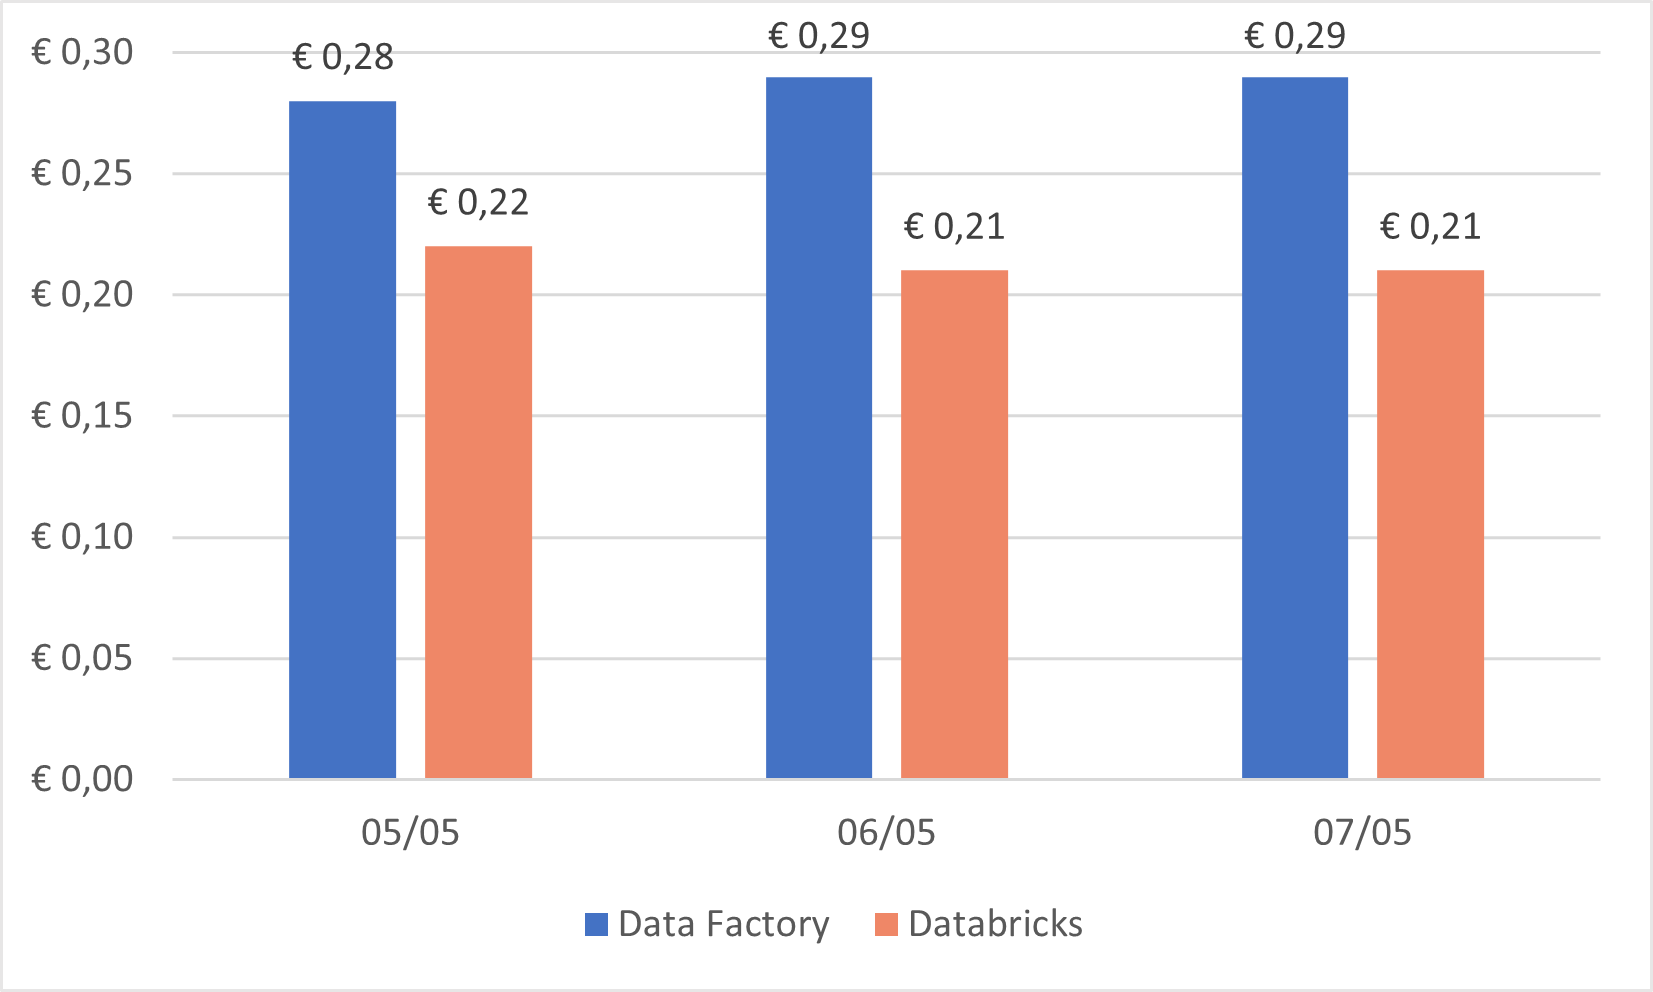
\includegraphics[width=0.8\textwidth]{./graphics/kosten/graf1.png}
    \caption{Prijzen voor pipeline met 4 Worker Cores + 4 Driver Cores}
\end{figure}
    
Deze grafiek toont de kosten per run van Data Factory en Databricks voor de pipeline met 4 Worker Cores + 4 Driver Cores over drie dagen: 5 mei, 6 mei en 7 mei. Uit de gegevens blijkt dat de kosten per run voor Data Factory op al deze dagen iets hoger liggen dan die van Databricks.

\begin{figure}[H]
    \centering
    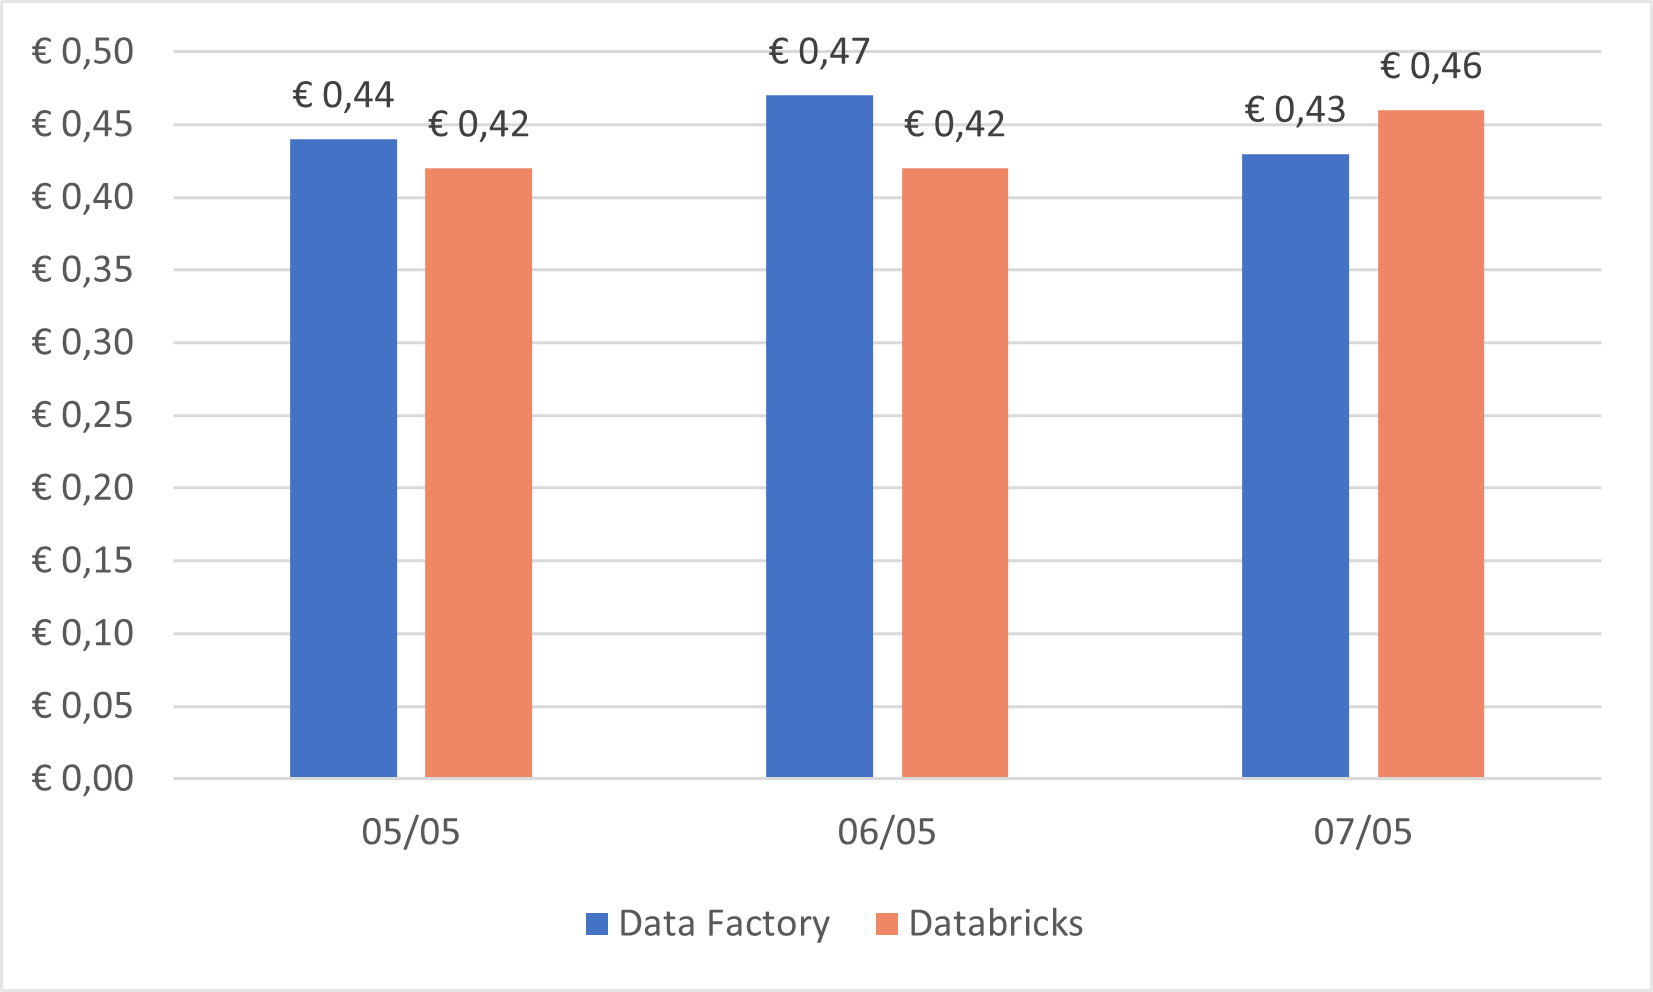
\includegraphics[width=0.8\textwidth]{./graphics/kosten/graf2.png}
    \caption{Prijzen voor pipeline met 8 Worker Cores + 8 Driver Cores}
\end{figure}

Ook hier liggen de kosten voor de pipeline met 8 Worker Cores + 8 Driver Cores iets hoger bij Data Factory, met uitzondering dat op 7 mei de kosten van databricks hoger lagen. Dit komt waarschijnlijk doordat de cluster startup tijd ook hoger lag.

\subsection{Performantie}

\begin{figure}[H]
    \centering
    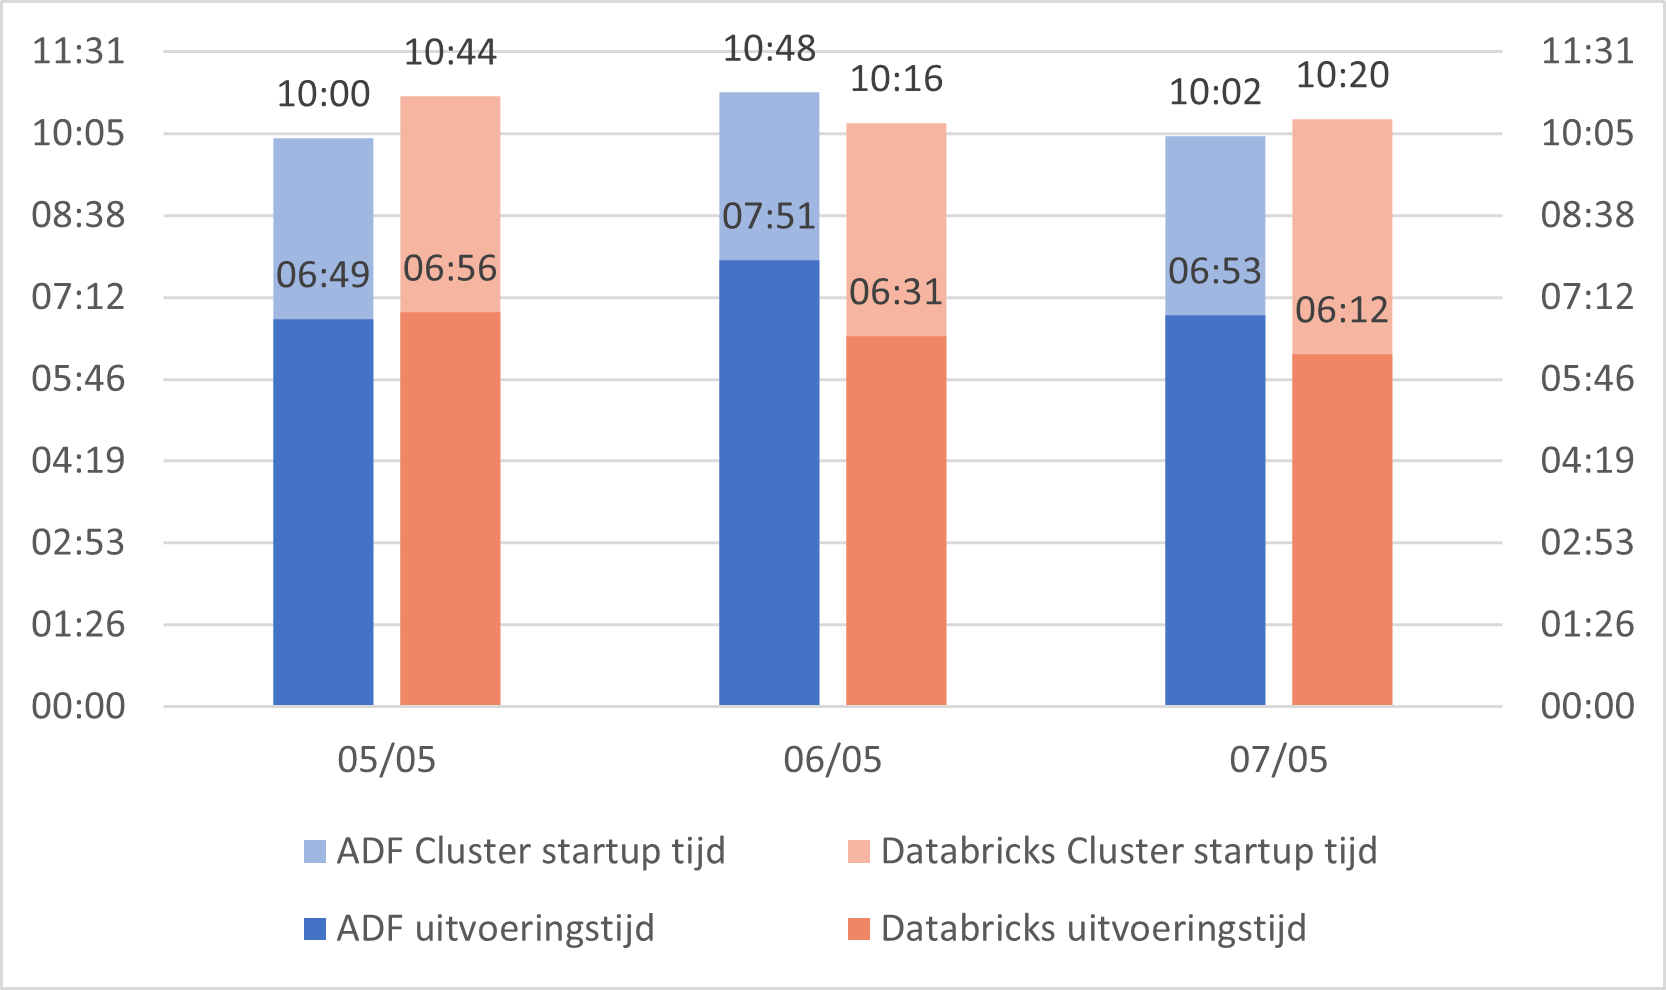
\includegraphics[width=0.8\textwidth]{./graphics/kosten/graf3.png}
    \caption{Uitvoeringstijden voor pipeline met 4 Worker Cores + 4 Driver Cores}
\end{figure}

In deze grafiek wordt per datum de uitvoeringstijd getoond voor de pipeline met 4 Worker Cores + 4 Driver Cores. De extra tijd die er bij komt is de cluster startup tijd die resulteert in een totale tijd. In de grafiek is het moeilijk te zien of Azure Data Factory of Azure Databricks de beste performantie heeft.

\begin{figure}[H]
    \centering
    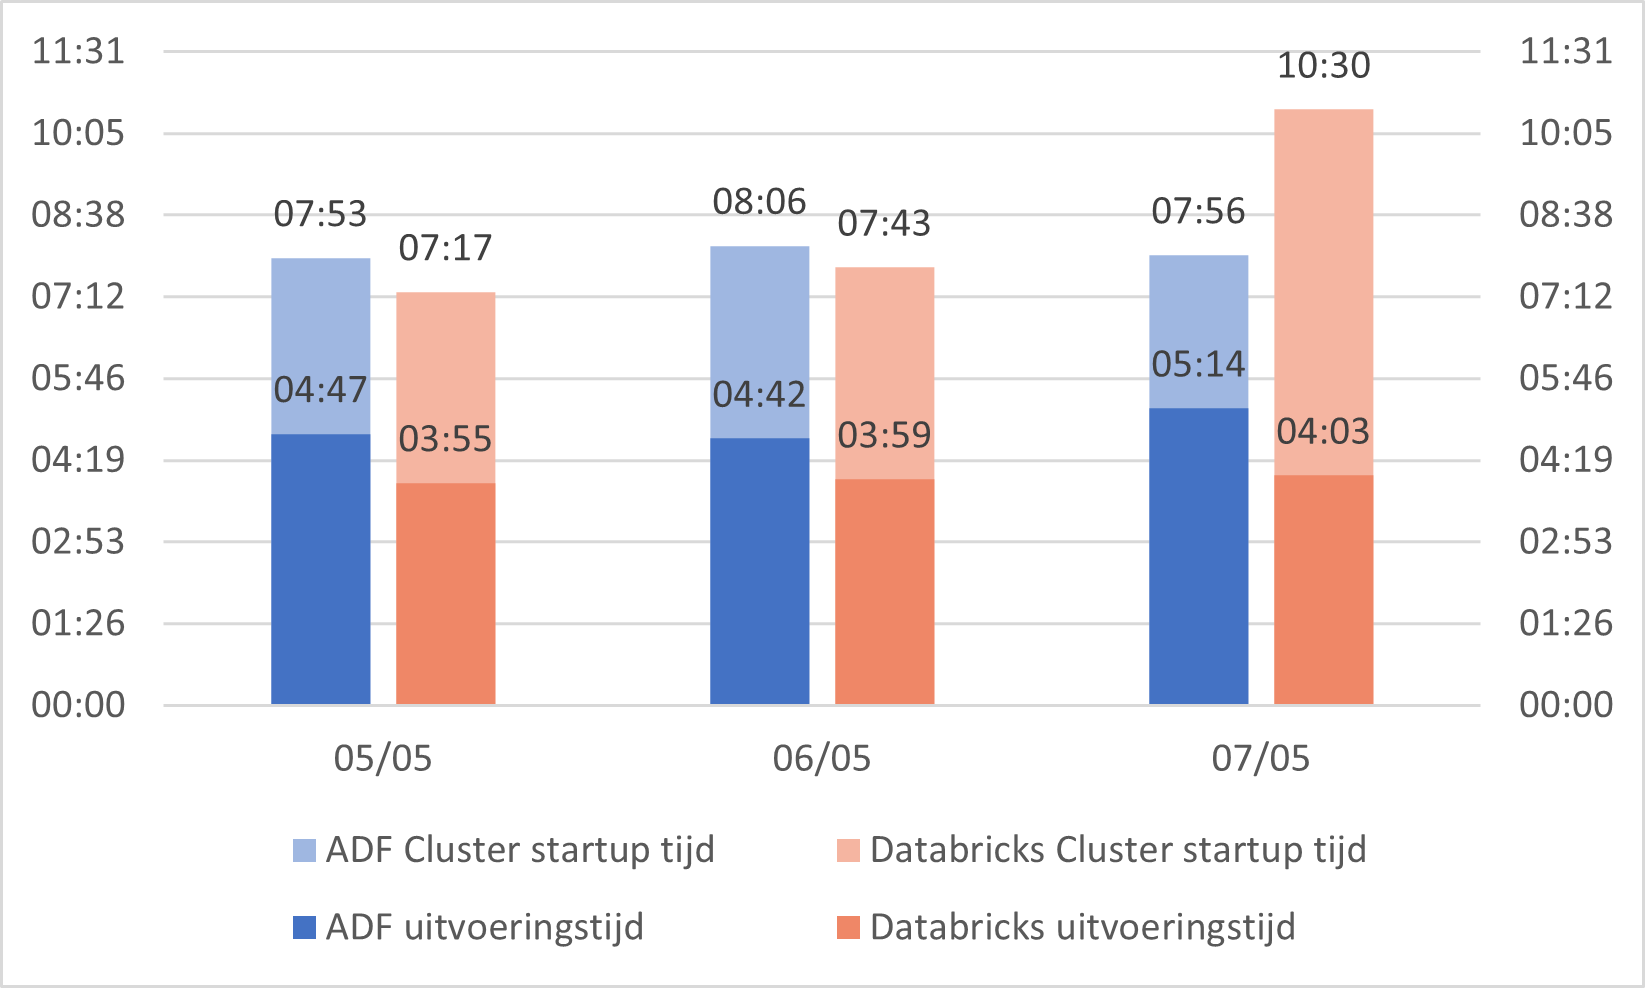
\includegraphics[width=0.8\textwidth]{./graphics/kosten/graf4.png}
    \caption{Uitvoeringstijden voor pipeline met 8 Worker Cores + 8 Driver Cores}
\end{figure}

Ook hier wordt de uitvoeringstijd per datum opnieuw getoond, maar deze keer voor de pipeline met 8 Worker Cores + 8 Driver Cores. Wanneer we kijken naar de uitvoeringstijd zien we dat Azure Databricks performanter is. Ook bij de totale tijd kunnen we dit zien, met uitzondering dat op 7 mei de cluster startup time hoger lag dan normaal. 

\begin{figure}[H]
    \centering
    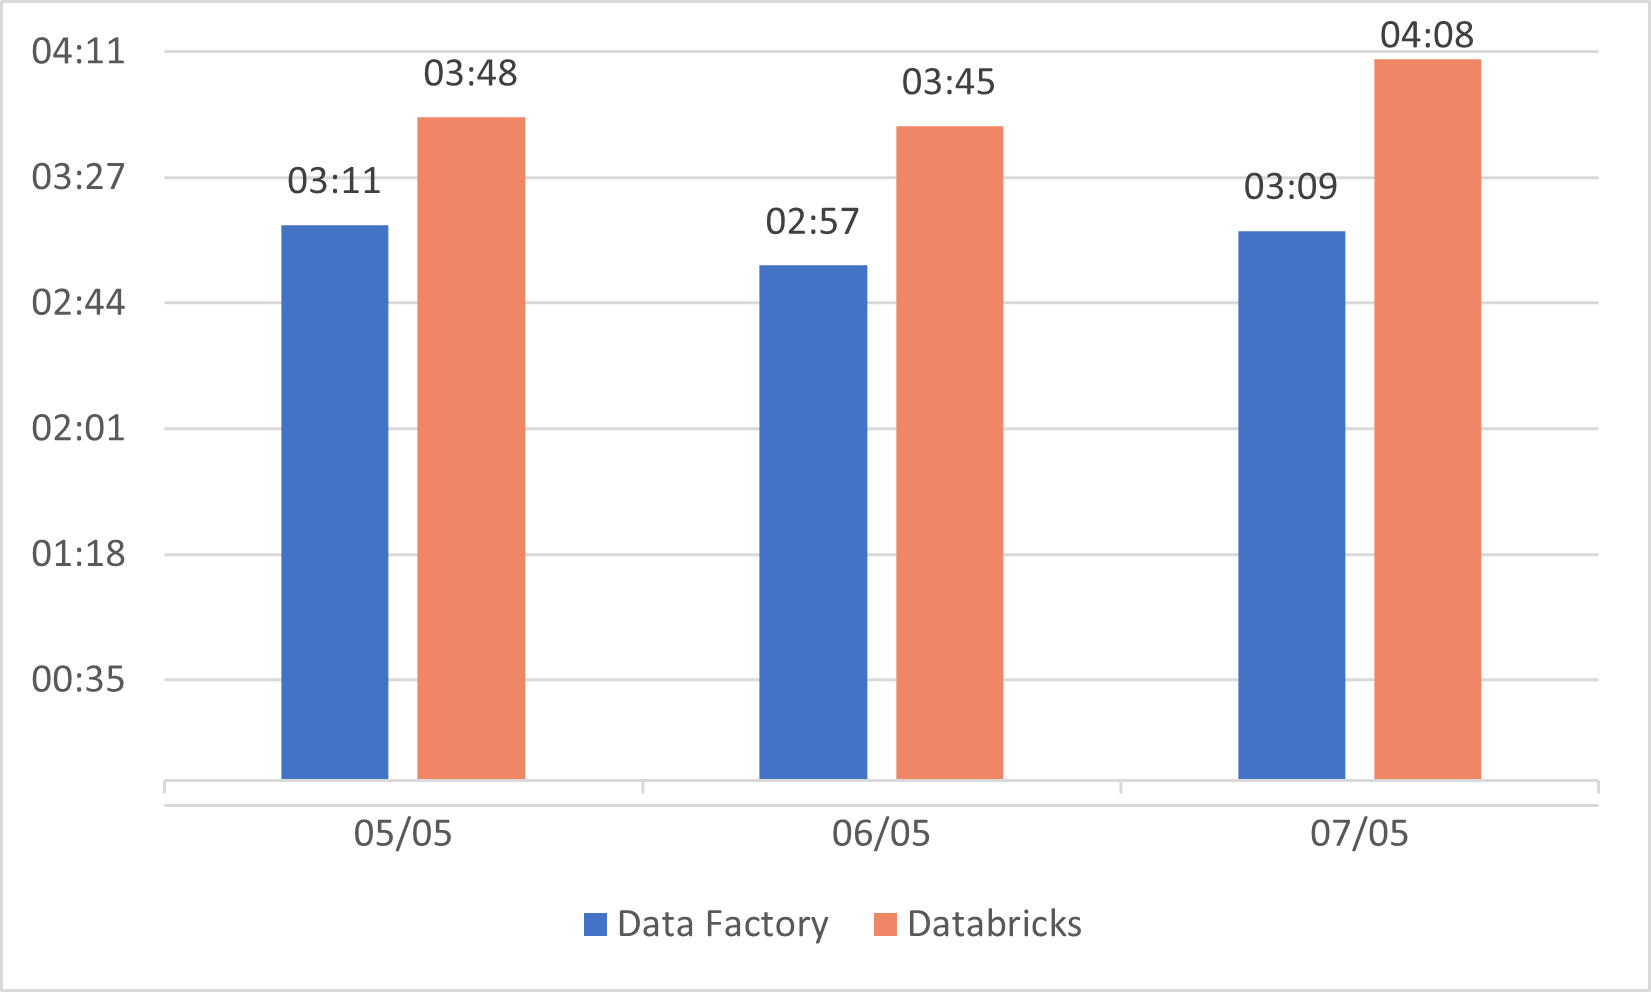
\includegraphics[width=0.8\textwidth]{./graphics/kosten/graf5.png}
    \caption{Cluster startup tijden voor pipeline met 4 Worker Cores + 4 Driver Cores}
\end{figure}

\begin{figure}[H]
    \centering
    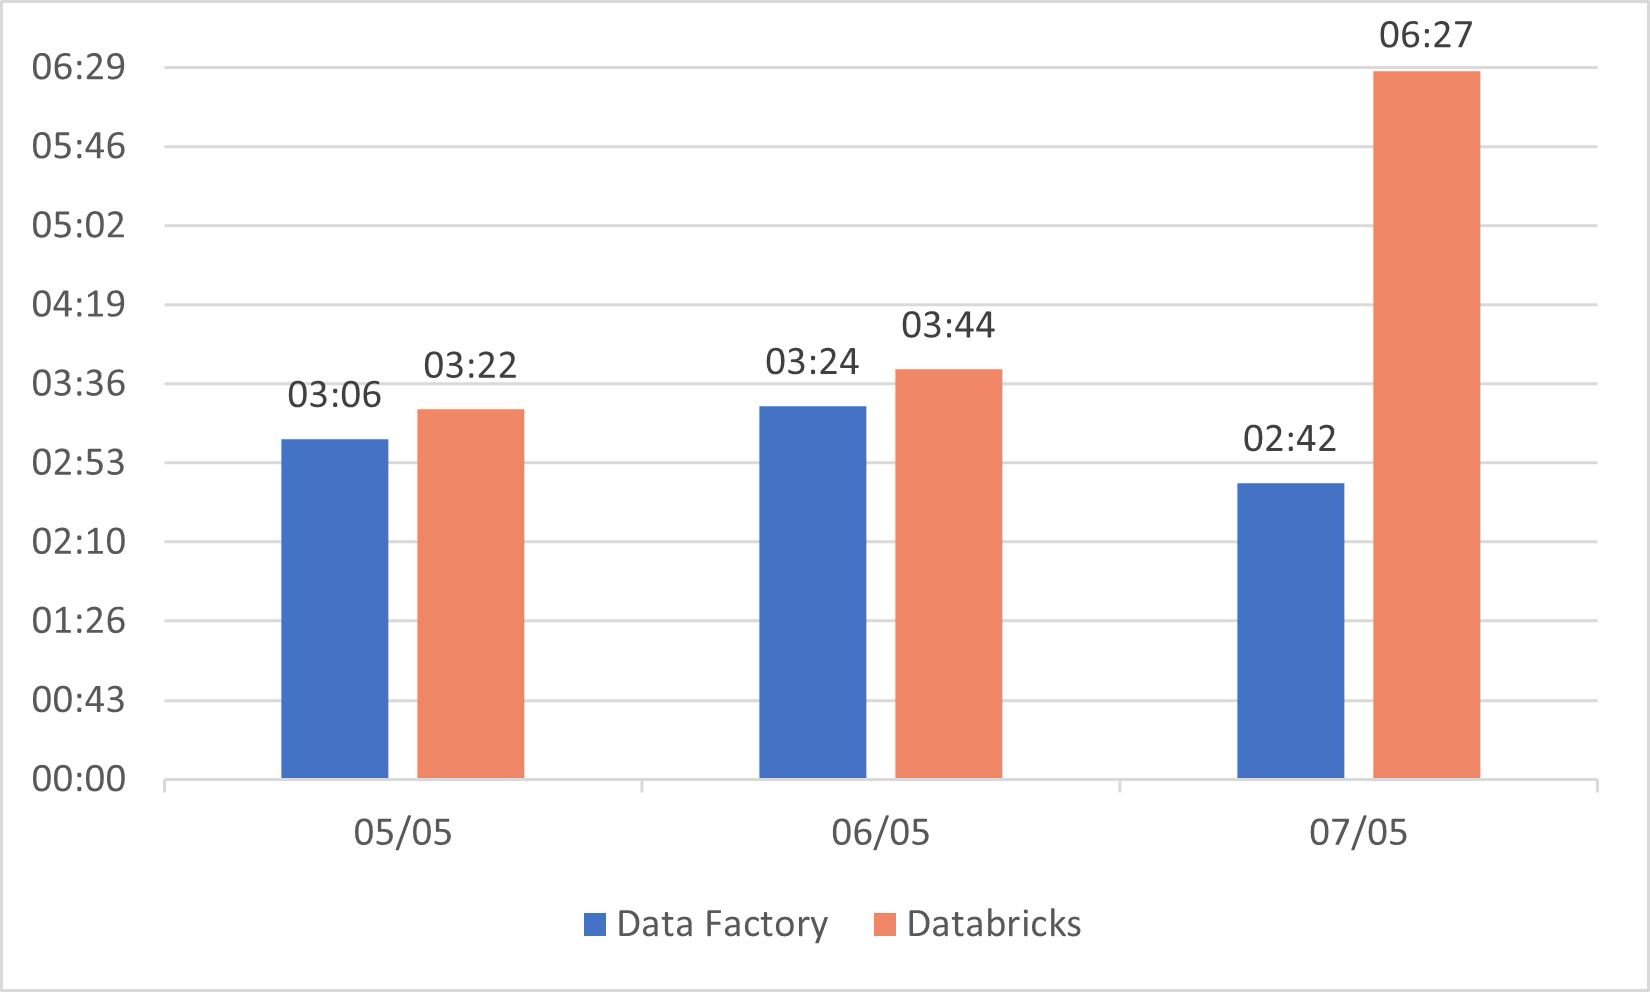
\includegraphics[width=0.8\textwidth]{./graphics/kosten/graf6.png}
    \caption{Cluster startup tijden voor pipeline met 8 Worker Cores + 8 Driver Cores}
\end{figure}

Wat wel opvallend is, is dat voor beide pipelines de cluster startup tijd voor Azure Data Factory opvallend lager is.